\section{Architectural goals}
For many libraries developed, it is a priority that the final product is easy to use, efficient and powerfull.  The same goals apply to the network library: It must be easy to use, the user should be able to start the library by just telling it what address it has, and it should be very easy to send a message, with nothing more than the data to send and an adress. Efficiency is more difficult, especially since the project requires using DTMF instead of an electric signal, but within that constraint, there is room for efficiency.
Also, the user-application thread will need to spend as little as possible execution time in the network library code, and do as little as possible memory management related to networking operations, as this will minimize faults in the library by user actions.



\subsection{Overall system architecture}
The general architecture of this library, as seen in Figure \ref{fig:general_architecture}, is to have one centralized backbone construct, which is the only part of the library to have any long term data storage and awareness of the network state. 
Within the backbone, resides a set of buffers used to store intermediate data and a set of layers, loosely corresponding to the layers of the osi model.
The layers are: Api, transport, datalink and physical.
The layers above the transport layer are deemed outside of the scope of this library, and instead an api layer is introduced to handle incoming and exiting data. Since we are not utilizing an electrical connection to transfer data, an extra layer is introduced below the physical layer, to handle playing and recording sound in a reliable way, this is the audio interface.









Layers are represented by an object that can encode or decode a sequence of bytes according to its rules. For instance the Data Link Layer can take a sequence of bytes representing a packet, and encode it to the form of frames.
However each of the different layer representation has no way of controlling when it is being used, no contextual information(i.e. knowledge of any other object in the system), and are therefore considered pure function objects.
The backbone monitors the buffers and the layers, and controls that transformation of data is done in a way that eliminates congestion as much as possible and ensures no data is lost. Since the backbone must be able to operate autonomously, it will be instantiated with its own execution thread. The data storage can then be regarded as an assembly line, where data is taken from one buffer, transformed and put into the next buffer, in order to apply all the necessary packaging that network communication requires, before the ''end data'' is sent to the audio library or the Api layer (in the case of sending and recieving data respectively).
Some of the layers might need attention based on other criteria than the condition of the buffers, it is the responsibility of the backbone to handle this as well.

\begin{figure}[htb]
	\begin{center}
	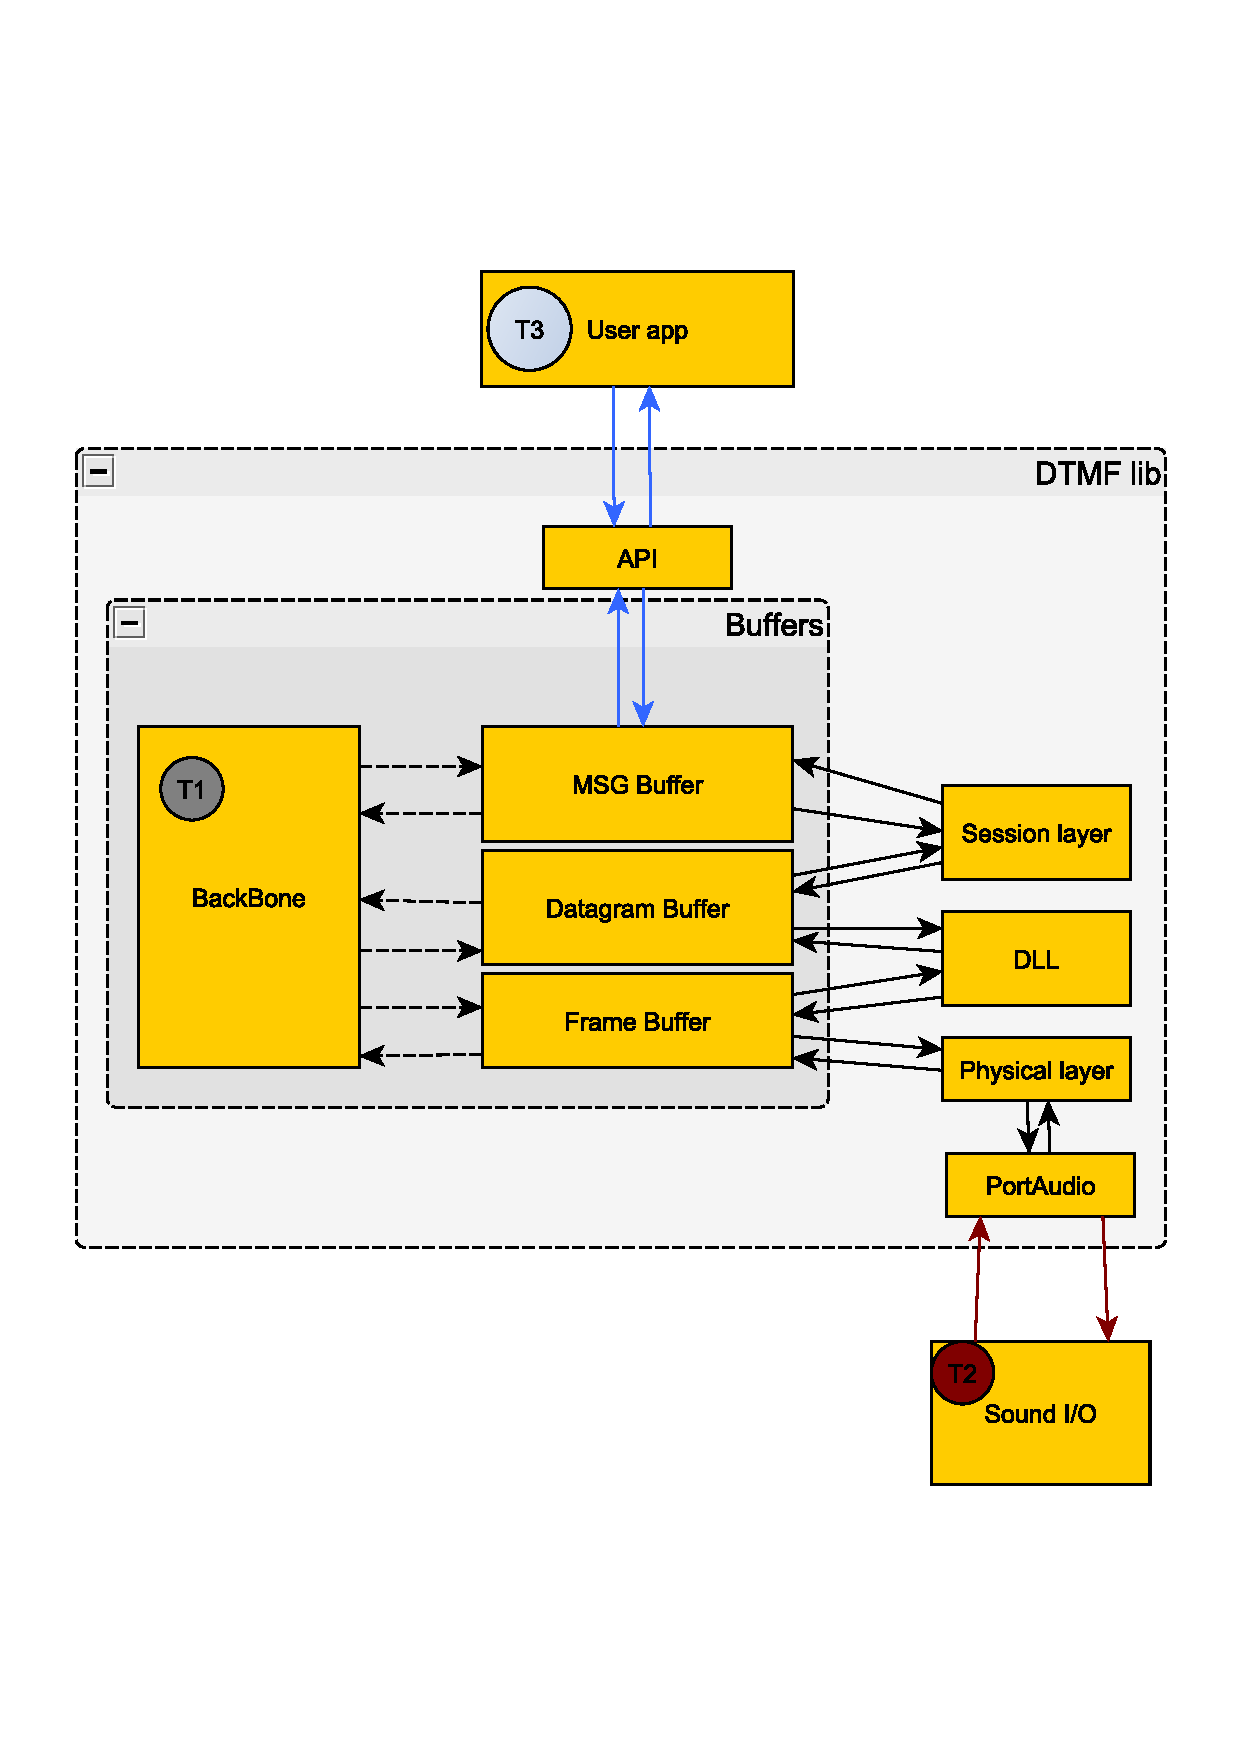
\includegraphics[scale=0.5,trim=0 130 0 130]{traadgraph.pdf}
	\caption{General DTMFLib architecture}
	\label{fig:general_architecture}	
	\end{center}
\end{figure}

\subsubsection{Facade class}
Any calls from the user goes through the API class and are passed on to the backbone. Data packages to and from the user are also buffered in the backbone to ensure low coupling. Since this is the only class the user can instantiate, it also has the responsibility of initializing the rest of the library upon creation.
When a user application wishes to send a message, the API will provide a ''message'' data holder, which can be filled and passed back to the API, this removes the need to do memory handling from the user application.
In order to receive messages from other systems, the user must register a callback function, that will be called by the network library when system has received a complete message. The lifetime of this message will be limited to the scope of the callback function.

\subsubsection{The layer classes}
The three layer classes reads data from a buffer, works on the data and writes it into the next buffer in the chain. Each layer may instantiate temporary internal buffers to store partially processed data between attention. Some of the layers will need to send a message to the layer before it, and when executing an encode or decode function, the layer is given access to both the appropriate send and receive buffers.


